\section{Vorgehen und Methoden}
Wie bereits in der Systembeschreibung beschrieben, wird der Fahrsimulator in 3 Hauptkomponenten unterteilt. Zum Fahrsimulator gehört ein UDP-Listener, ein Szenen-Manager und das Hauptprogramm. Da die Verbindung zwischen dem Cockpit und dem Fahrsimulator mit einer Netzwerkschnittstelle realisiert wird, ist es möglich die Anbindung an das Cockpit und den Fahrsimulator phisikalisch auf zwei Rechnern zu betreiben. Eine weiter Lösung hätte mit dem Ogre-Framework (Siehe Anhang D?) realisiert werden können. Dieses Framework bietet umfassende Lösungen um Steuerradär und Pedalen, wie sie in userem Cockpit vorhanden sind, anzusteueren.\\
Da die 3D-Umgebungen mit fortscheitendem Projekt zunimmt, könnte die Rechenleistung der momentan verwendeten Maschiene zu einem späteren Zeitpunkt nicht mehr ausreichen. Die Folgen von ungenügender Leistung können unregelmässige Bewegungen (Lags) in der virtuellen Umgebung sein oder es kann sogar bis zum Absturz des gesamten Programms führen. \\
Dieses Problem hat zur Folge, dass der Fahrsimulator einer hohen Portierbarkeitanforderung genügen muss. Damit ist die Variante mit der Netzwerkschnittstelle für das Fahrsimulatorprojekt geeignet. Die andere Variante wird verworfen.
\subsection{LabView modifizierung}
Es existiert bereits ein LabVIEW-Programm das die Eingaben im Cockpit einliest. Dieses Programm wird so erweitert das diese Eingaben in Form von definierten Parameter als UDP-Packet permanent gesendet werden. Zusätzlich wird ein weitert UDP-Socket eingerichtet um Packete die vom Fahrsimulator gesendet werden zu empfangen. Die Daten der empfangenen Packete werden von LabVIEW in ein Log-File gespeichert. 
% ev Bild
\subsection{UDP-Socket}
Die Paramter werden vom LabVIEW-Programm permanent gelesuen und mindestens 50 mal pro Sekunde wird ein UDP-Packet gesendet. Um die Zeit zwischen der Eingabe des Probanden und dem ragierne des Fahrzeuges im Simulator möglichst tief zu halten, müssen ankommende Packete sofort gelesen werden. Unwichtig ist jedoch das jedes Packet empfange wird oder das die Packete in der gleichen Reihenfolge ankommen wie sie gesendet wurden. Das UDP-Protokoll gewährleistet genau diese Eigenschaften. \\

\begin{figure}[H]
\centering 
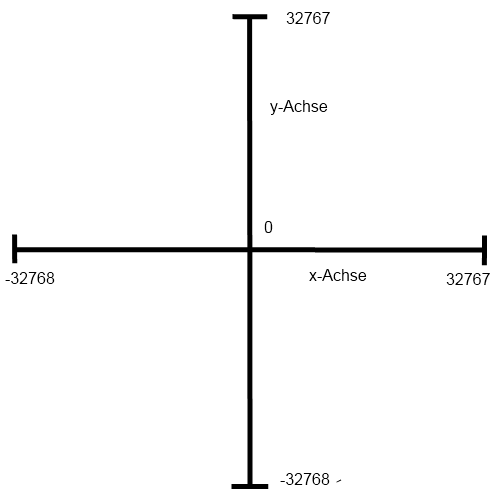
\includegraphics[scale=0.5]{src/koordinatensystem.png}
\caption{Koordinatensystem} % Titel der Grafik
\label{Koordinatensystem} % Labelname
\end{figure}

Die Daten die vom LabVIEW empfangen werden, sind in erster Linie Parameter die den Zustand der Pedalen und des Steuerrades representieren. Die beiden Pedalen werden in einem Koordinatensystem wie in Abbildung \ref{Koordinatensystem} auf der y-Achse abgebildet. Die positive y-Richtung quantifiziert das Gas und die negative y-Richtung das Bremspedal. Die intensität beider Pedalen wird durch 32767 bzw. 32768 ganzzahlige Werte identifiziert. Wenn also keins der beiden Pedalen gedrückt ist, wird dies durch den y-Wert 0 dargestellt. Ein voll gedrücktes Gaspedal entspricht dem y-Wert 32767 und dementsprechend ein voll gedrücktes Bremspedal dem Wert -32768. Der x-Wert im Koordinatensystem quantifiziert den Einschlagswinkel des Steuerrades. Ist das Steuerrad in der neutralen Stellung, entspricht dies dem x-Wert 0. Wenn das Steuerrad vollständig nach rechts eingeschlagen ist, wird dies durch den positiven x-Wert 32767 identifiziert. Umgekehrt wird ein vollständiger Einschlag nach links durch den negiativen x-Wert -32768 identifiziert. Es können zusätzlich weitere Parameter, wie Tastendrücke am Steuerrad, übermittlet werden, wenn dies erforderlich sein sollte. Zusätzlich zu den Parametern des Cockpits wird von LabVIEW auch noch ein Timestamp gesendet. Der Timestamp wird von UDP-Listener empfangen und nach dem abspeichern der Parameter wieder zurückgeschikt. Somit kann festgestellt werden wieviel Verzögerung die Netzwerkschnittstelle verursacht. \\
Da das LabVIEW-Programm und der Simulator nicht synchronisiert sind, wird der DP-Listener dazu verwendet dies zu überbrücken. Der UDP-Listener speicher alle Parameter in Variabeln ab. Diese Variabeln werden vom Hauptprogramm ausgelesen und interpretiert. Dieses auslesen der Variabeln erfolgt nun synchron, da das Hauptprogramm nur dann Daten vom UDP-Listener liest wenn dieses dazu bereit ist.

\subsection{Virtual Reality}
\subsection{Hautpprogramm}

\lstinputlisting{listings/Karte.java}


%Sequenzdiagramm
%Blockdiagramm

